\documentclass[a4]{article}
\usepackage{amssymb}
\usepackage{amsmath}
\usepackage{bm}
\usepackage{graphicx}
\usepackage{physics}
\usepackage[strings]{underscore}

\DeclareMathOperator*{\argmax}{argmax}
\DeclareMathOperator*{\argmin}{argmin}


\newtheorem{defn}{Definition}

%opening
\title{ Notes on Sampling: Basics \& MCMC}
\author{Shoichiro Yamanishi}

\begin{document}

\maketitle

%\begin{abstract}
%\end{abstract}


\section{Overview}
This is a personal expository material on sampling mainly 
for my future self to quickly refresh the topics.
It also contains explanations to the topics that are unclear to me in the books and articles.
The following topics are covered.

\begin{itemize}
\item Basic sampling : from uniform distribution to a particular distribution.
\item Rejection sampling
\item Importance sampling
\item Uni/Bivariate Gaussian Distribution : Box-Muller algorithm
\item Univariate Gaussian Distribution with rejectio sampling : Ziggurat algorithm
\item Multivariate full-covariance Gaussian distribution
\item MCMC (Metropolis-Hastings)
\item Gibbs Sampling
\item MCMC with Hamiltonian dynamics
\end{itemize}



\section{Why Sampling?}
Sampling is an effective means to numerically calculate expectations of random variables over 
a given distributoin.
\begin{equation}
\mathbb{E}_{\bm{x}\sim p(\bm{x})}\left[f(\bm{x})\right] = \int f(\bm{x})p(\bm{x})d\bm{x}
\approx \frac{1}{L}\sum_{i=1}^{L}f(\bm{x}_i)\label{eq:1}
\end{equation}
where $\bm{x}_i$ are i.i.d. drawn from the given $p(\bm{x})$.



\subsection{Theoretical Back-up}
Barber \cite{Barber2011} briefly touches on it in Chap 27.
We denote the RHS of equation \ref{eq:1} by $\bm{\mu}_f$.
We take the limit of $\bm{\mu}_f$ as in $L\rightarrow \infty$, then:
\begin{equation}
\begin{aligned}
\mathbb{E}\left[\bm{\mu}_f\right]
&=
\mathbb{E}\left[\frac{1}{L}\sum_{i=1}^{L}f(\bm{x}_i)\right]\\
&= \frac{1}{L}\mathbb{E}\left[\sum_{i=1}^{L}f(\bm{x}_i)\right]\\
&= \frac{1}{L}\mathbb{E}\left[L f(\bm{x})\right]
\:\text{because}\:\bm{x}_i\:\text{are i.i.d.}\\
&= \mathbb{E}\left[f(\bm{x})\right]\\
\end{aligned}
\end{equation}
and the variance of each sampled $f(\bm{x}_i)$ is
\begin{equation}
\begin{aligned}
\mathbb{E}\left[
    \frac{1}{L}\sum_{i=1}^{L}\left( f(\bm{x}_i) - \bm{\mu}_f \right)^2
\right]
&= \left( \frac{L - 1}{L} \right)
\left( \mathbb{E}\left[ f(\bm{x}_i)^2 \right] - 
       \mathbb{E}\left[ f(\bm{x}_i) \right]^2 \right)\\
&= \left( \frac{L - 1}{L} \right)\mathbb{E}\left[
\left( f(\bm{x}_i) - \mathbb{E}\left[ f(\bm{x}_i) \right] \right)^2
\right]\label{eq:3}\\
\end{aligned}
\end{equation}
so the variance of sampled $f(\bm{x}_i)$ approaches the variane of $f(\bm{x})$
according to $p(\bm{x})$ as $L\rightarrow \infty$.
Equation \ref{eq:3} comes from a similar argument for PRML \cite{bishop2007} (1.58), for which
I have arranged a separate document titled \textit{PRML (1.58) : Why $\mathbb{E}[\sigma_{sample}^2] = \frac{N-1}{N}\sigma^2$ ?} for deduction.

\textbf{NOTE} The equation (27.1.4) in Barber \cite{Barber2011} quoted following is wrong.
\begin{equation}
\begin{aligned}
\langle \hat{f}^2 \rangle - \langle \hat{f} \rangle^2 = \frac{1}{L}
\left( \langle f^2(x)\rangle_{p(x)} - \langle f(x) \rangle^2_{p(x)} \right)\\
\end{aligned}
\end{equation}
According to this equation, the variance vanishes as $L\rightarrow \infty$, which is
clearly wrong. The deductions around (1.54) - (1.58) in PRML\cite{bishop2007} gives the correct argument
for a similar situation. PRML gives an argument for $\bm{x}$ but it can be easily applicable
to $f(\bm{x})$.



\section{Basic Univariate Sampling}
Section 11.1. of PRML\cite{bishop2007} gives a good overview, but I have made further annotation as it was still not clear to me.
We assume a mechanism to draw a sample $x_i$ from a uniform distribution is available.
\begin{equation}
\begin{aligned}
p(x) = \begin{cases}
1 & \text{if}\: 0 \le x \le 1\\
0 & \text{otherwise}
\end{cases}
\end{aligned}
\end{equation}

We want to draw samples $y_i$ from a probability density distribution $p(y)$,
 which is differentiable everywhere.
We want to find a function $x \mapsto y,\:\: y = h(x)$ so that we can draw $x$ and then
convert it to $y$ that follows the distribuion $p(y)$.
We show $y = h(x)$ is an inverse of the cummulative distribution function of $P(y)$.

To see this, for $0\le x \le 1$, 
\begin{equation}
\begin{aligned}
p(x) = p(y)\left|\frac{dy}{dx}\right|=1
\end{aligned}
\end{equation}
so \begin{equation}
\begin{aligned}
p(x)dx = p(y)dy
\end{aligned}
\end{equation}
The cummulative distribution function $P(x)$ is
\begin{equation}
\begin{aligned}
P(x) = \int_{-\infty}^{x}p(x)dx = x, \:\:x \le 1\label{eq:8}
\end{aligned}
\end{equation}
and the cummulative distribution function $P(y)$ is
\begin{equation}
\begin{aligned}
P(y) = \int_{-\infty}^{y}p(y)dy &= \int_{-\infty}^{h^{-1}(y)}p(x)dx
\:\:\: \text{(from equation \ref{eq:8})}\\
&= \int^{h^{-1}(y)}_{-\infty}dx = h^{-1}(y) 
\end{aligned}
\end{equation}
so $h(x) = P^{-1}(y)$.
The following charts give you some intuition into this conversion.
This is basically annotated and clearer version of Figure 11.2 in PRML \cite{bishop2007}.

\begin{figure}
\centering
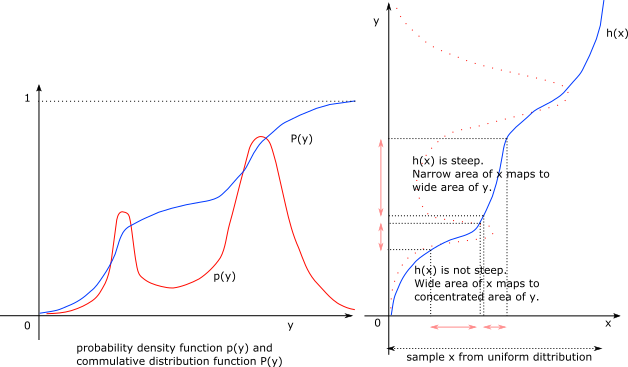
\includegraphics[width=12cm]{basic_sampling.png}
\caption{Graphical Interpretation of h(x)}
\label{fig:basic_sampling}
\end{figure}


\section{Rejection Sampling}
Please see 11.1.2 of PRML \cite{bishop2007}. Following is a quick refresher.
Rejecton Shsampling is applicable for the following case.
\begin{itemize}
\item $p(\bm{z})$ is of low dimension.
\item evaluation of an unnormalized $\hat{p}(\bm{z})$ tractable.
\item easy to find a proposal distribution $q(\bm{z})$ not far from $p(\bm{z})$,
and for all $\bm{z}$ in the domain there is $K$ such that $Kq(\bm{z}) \ge \hat{p}(\bm{z})$.
\end{itemize}

And the following are the steps.
\begin{itemize}
\item Draw $\bm{z}^*$ from $q(\bm{z})$.
\item Draw $u^*$ from the uniform distribution in $[0, Kq(\bm{z}^*)]$.
\item Accept $\bm{z}^*$ if $u^* \le p(\bm{z}^*)$. Discard it otherwise.
\end{itemize}
See figure 11.4 in pp 529 of PRML for the reason why it works.
This is not suitable if the area for rejection is too big.


\section{Importance Sampling}
Please see 11.1.4 of PRML \cite{bishop2007} for more info as it is well written.
This does not draw samples directly but approximate expectations using a proposal distribution.
you don't need actual samples but only the approximation to some expectations.
Imporance sampling is applicable for the following case.
\begin{itemize}
\item $p(\bm{z})$ is of low dimension.
\item evaluation of an unnormalized $\hat{p}(\bm{z})$ tractable.
\item you don't need samples but only approxmiation to some expectations.
\end{itemize}
The following is the basic idea.
\begin{equation}
\begin{aligned}
\mathbb{E}_{\bm{z}\sim p(\bm{z})}\left[f(\bm{z})\right] &= \int f(\bm{z})p(\bm{z})d\bm{z}\\
&= \int f(\bm{z})\frac{p(\bm{z})}{q(\bm{z})}q(\bm{z})d\bm{z}
\:\:\:\:\:\:q(\bm{z}) \text{ is a proposal distribution.}\\
&\approx \frac{1}{L}\sum_{i=1}^L \left(f(\bm{z}_i)\frac{p(\bm{z}_i)}{q(\bm{z}_i)}\right)
\:\:\:\:\:\:\bm{z}_i \sim q(\bm{z})
\end{aligned}
\end{equation}
And we can use unnormalized version as follows.
\begin{equation}
\begin{aligned}
\mathbb{E}_{\bm{z}\sim p(\bm{z})}\left[f(\bm{z})\right]
&\approx \frac{Z_q}{Z_p}\frac{1}{L}
    \sum_{i=1}^L \left(f(\bm{z}_i)\frac{\hat{p}(\bm{z}_i)}{\hat{q}(\bm{z}_i)}\right)
\end{aligned}
\end{equation}
where $p(\bm{z})=\frac{1}{Z_p}\hat{p}(\bm{z})$, and $q(\bm{z})=\frac{1}{Z_q}\hat{q}(\bm{z})$, and
$\frac{Z_q}{Z_p}$ can be approximated as follows.
\begin{equation}
\begin{aligned}
Z_p &= \int \hat{p}(\bm{z})d\bm{z}\\
    &= \int \frac{\hat{p}(\bm{z})}{q(\bm{z})}q(\bm{z})d\bm{z}\\
    &= \int Z_q \frac{\hat{p}(\bm{z})}{\hat{q}(\bm{z})}q(\bm{z})d\bm{z}\\
    &= Z_q \int\frac{\hat{p}(\bm{z})}{\hat{q}(\bm{z})}q(\bm{z})d\bm{z}\\
    &\approx Z_q \sum_{i=1}^L \left(\frac{\hat{p}(\bm{z}_i)}{\hat{q}(\bm{z}_i)}\right)
\:\:\:\:\:\:\bm{z}_i \sim q(\bm{z})\\
\end{aligned}
\end{equation}


\section{Uni/Bivariate Gaussian Distribution : Box-Muller Algorithm}
We can't simply draw a sample from $\mathcal{N}(0,1)$ because the cummulative probability function
of the normal distribution, expressed by
$P(x) = \frac{1}{2}\left[ 1 + \text{erf}\left(\frac{x}{\sqrt{2}}\right) \right]$,
$\text{erf}(x) = \frac{2}{\sqrt{\pi}}\int_0^x e^{-t^2}$dt
is not tractable, and hence inverse $x = P^{-1}(y)$ is difficult to compute.

Box-Muller algorithm \cite{BoxMull58} draws a pair of samples $(x_1, x_2)$ using some clever tricks.
There are two flavors of Box-Muller Algorithm: $\chi^2$-form and the polar form.
11.1.1 of PRML \cite{bishop2007} explains the polar form. Here we describe the $\chi^2$-form, which is
simpler and more elegant.

First, we draw $z_1$ and $z_2$ from a uniform distribution in $[0,1]$, and
\begin{equation}
\begin{aligned}
x_1 &= \sqrt{-2\ln z_1}\cos(2\pi z_2)\\
x_2 &= \sqrt{-2\ln z_1}\sin(2\pi z_2)
\end{aligned}
\end{equation}

Then we obtain samples $x_1$ and $x_2$ drawn from $\mathcal{N}(0,1)$.

Here's the derivation.
Assume $x_1$ and $x_2$ are drawn from $\mathcal{N}(0,1)$, and let
$$R^2 = x_1^2 + x_2^2 = -2\ln z_1.$$
Then $R^2$ follows the $\chi^2$-distribution of degree 2.
The PDF of $\chi^2$-distribution is 
$$p(x) = \frac{1}{2^{k/2}\Gamma(k/2)}x^{k/2-1}e^{-x/2},$$
and when the degree $k=2$,  it is
simply an exponential distributoin $\frac{1}{2}e^{-x/2}$, so
$p(R^2) = \frac{1}{2}e^{-R^2/2}$, which suggests R follows a normal distribution.
To be precise,
\begin{equation}
\begin{aligned}
z_1 &= \exp(\frac{x_1^2 + x_2^2}{2})
\end{aligned}
\end{equation}
and
\begin{equation}
\begin{aligned}
\frac{x_2}{x_1} &= \tan(2\pi z_2)\:\:\:\:\:\:\:\: z_2 = \frac{1}{2\pi}\tan^{-1}(\frac{x_2}{x_1})
\end{aligned}
\end{equation}
Taking the partial derivatives of them,
\begin{equation}
\begin{aligned}
\frac{\partial z_1}{\partial x_1} = - x_1 \exp(\frac{x_1^2 + x_2^2}{2})\\
\frac{\partial z_1}{\partial x_2} = - x_2 \exp(\frac{x_1^2 + x_2^2}{2})\\
\end{aligned}
\end{equation}
and ($\frac{d}{dx}\tan^{-1}(x) = \frac{1}{x^2 + 1}$),
\begin{equation}
\begin{aligned}
\frac{\partial z_2}{\partial x_1} &= \frac{1}{2\pi}\frac{-x_2/x_1^2}{(x_2/x_1)^2+1}
= - \frac{1}{2\pi}\frac{x_2}{(x_1^2+x_2^2)}\\
\frac{\partial z_2}{\partial x_2} &= \frac{1}{2\pi}\frac{x_1^{-1}}{(x_2/x_1)^2+1}
= \frac{1}{2\pi}\frac{x_1}{(x_1^2+x_2^2)}\\
\end{aligned}
\end{equation}
and from the conversion formula of the PDF,
\begin{equation}
\begin{aligned}
p(x_1, x_2) 
&= p(z_1, z_2)\left| \frac{\partial(z_1, z_2)}{\partial(x_1, x_2)} \right|\\
&= p(z_1)p(z_2)\left|
    \frac{\partial z_1}{\partial x_1}\frac{\partial z_2}{\partial x_2}
    - \frac{\partial z_2}{\partial x_1}\frac{\partial z_1}{\partial x_2}
\right|\\
&= \left|
-\frac{1}{2\pi}\frac{x_1^2}{x_1^2 + x_2^2}\exp\left( -\frac{x_1^2 + x_2^2}{2}\right)
-\frac{1}{2\pi}\frac{x_2^2}{x_1^2 + x_2^2}\exp\left( -\frac{x_1^2 + x_2^2}{2}\right)
\right|\\
&= \left|
-\frac{1}{2\pi}\frac{x_1^2+ x_2^2}{x_1^2 + x_2^2}\exp\left( -\frac{x_1^2 + x_2^2}{2}\right)
\right|\\
&= \left|
-\frac{1}{2\pi}\exp\left( -\frac{x_1^2}{2}\right)\exp\left( -\frac{x_2^2}{2}\right)
\right|\\
&=
\frac{1}{\sqrt{2\pi}}\exp\left( -\frac{x_1^2}{2}\right)
\frac{1}{\sqrt{2\pi}}\exp\left( -\frac{x_2^2}{2}\right)\\
&= \mathcal{N}(x_1;0,1)\mathcal{N}(x_2;0,1)\\
\end{aligned}
\end{equation}



\section{Univariate Gaussian Distribution : Ziggurat Algorithm}
This is a combination of table look-up and rejection sampling for speed.
This framework is applicable to any monotone-decreasing or increasing PDF.
Here we apply the positive half of the unit normal distribution. $\mathcal{N}(x;0,1), x \ge 0$.


Beforehand, the PDF is split into strips of equal area horizontally.
See Figure \ref{fig:ziggrat_layers}.
Each Strip consists of the red rectangle region and the yellow region to the right,
except for the top strip ($R9$ in the example), which consists of a yellow region only,
and the bottom strip $R0$, which is not rectanglar but horizontall unbounded.
For $R0$, the gray rectangle to the right has the same height as $R0$ and the same area as the
yellow unbounded tail.

Each sampling of $x_i$ goes through the following steps.
\begin{itemize}
\item draw a strip $RS_i$ from a discrete uniform distribution.
\item draw a horizontal extent $x_i$ from a uniform distribution $[0, x_{S_i}]$.
\item if $x_i$ falls into the red region, then accept $x_i$.
\item otherwise, if $RS_i$ is not the bottom strip, then draw a horizontal extent $y_i$ from 
$[y_{S_i}, y_{S_i+1}]$ and if $p(x_i) \ge y_i$, accept $x_i$. Reject it otherwise.
\item if $RS_i$ is the bottom strip and if $x_i$ is in the gray region $[x_1, x_0]$, then we
ignore $x_i$ and go through the following extra steps.
\end{itemize}

The extra steps for the bottom unbounded tail are as follows.
Here I follow the origina article  \cite{ziggurat_1963}, which is a declassified defense document,
as its explanation is the clerest for me.
As the horizontal extent is unbounded, we can't draw $x_i$ from a uniform distribution.
We reverse the role of $x$-axis and $p(x)$-axis as in Figure \ref{fig:ziggrat_R0}.
In this figure, $a$ corresponds to $x_1$ in Figure \ref{fig:ziggrat_layers}.
And we introduce a new variable $U_1$ for the horizontal axis.
And we scale the horizontal axis by $\frac{1}{\frac{1}{\sqrt{2\pi}}\exp{-\frac{a}{2}}}$ so that
the range of $U_1$ becomes $[0,1]$. (The original article \cite{ziggurat_1963} is made that way, so I follow it.)
Then the curve is expressed by $x = \sqrt{a^2 - 2\ln(U_1)}$.

\begin{itemize}
\item draw a sample $U_1^*$ from a uniform distribution from $[0,1]$.
\item $a^* = \sqrt{a^2 - 2\ln(U_1^*)}$.
\item apply rejection sampling. Accept $a^*$ with the probability of $a/a^*$. For that draw another
sample $U_2$ from a uniform distribution from $[0,1]$, and accept $a^*$ if $U_2 \le a/a^*$.
\end{itemize}


\begin{figure}
\centering
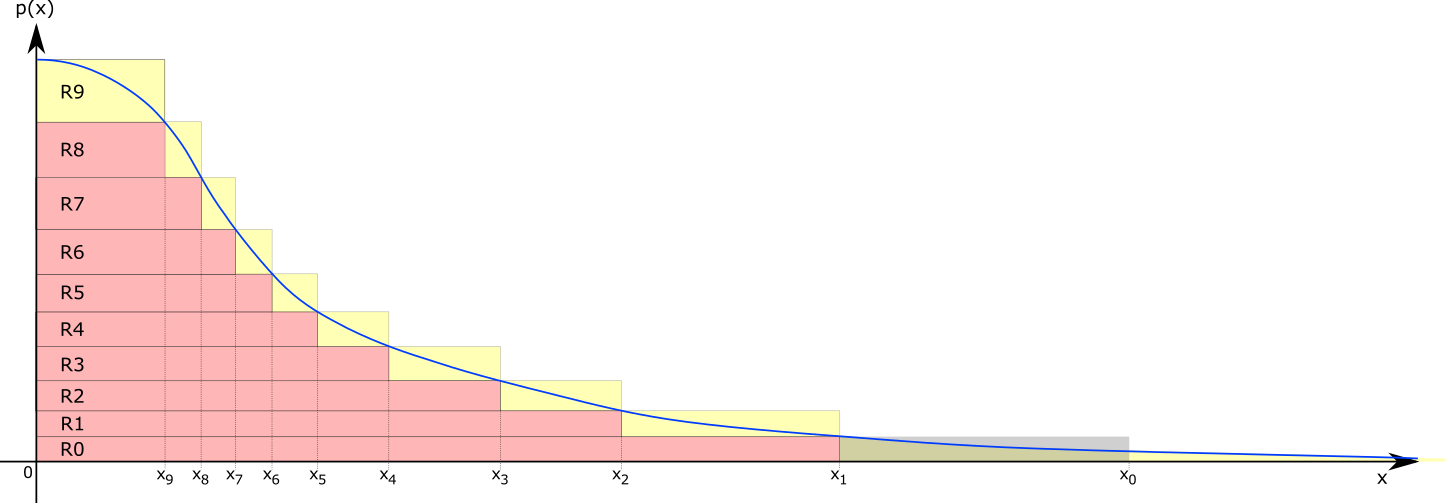
\includegraphics[width=14cm]{ziggurat_layers.png}
\caption{Horizontal Layers of Equal Area}
\label{fig:ziggrat_layers}
\end{figure}

\begin{figure}
\centering
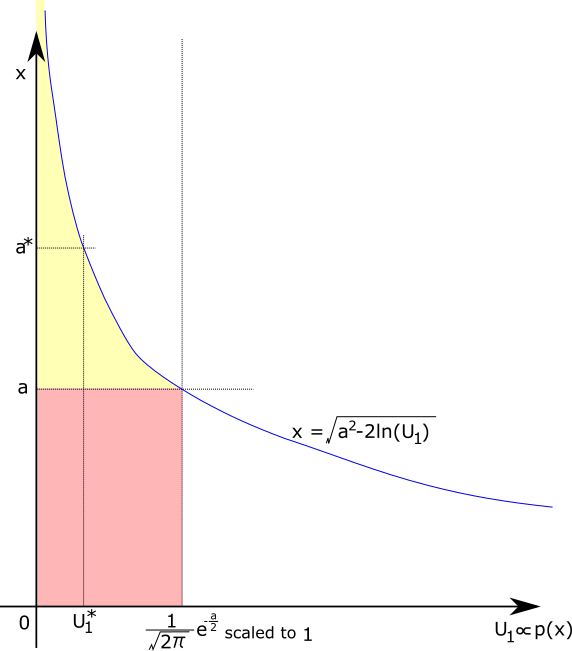
\includegraphics[height=8cm, width=8cm]{ziggurat_R0.png}
\caption{Layer R0 Arranged Upright and Scaled Horizontally such that $\frac{1}{\sqrt{2\pi}}
\exp(-\frac{a^2}{2}) = 1$.}
\label{fig:ziggrat_R0}
\end{figure}



\section{Multivariate Full-Covariance Gaussian Distribution}
To draw a sample $\bm{x} \in R^N, \bm{x} \sim \mathcal{N}(\bm{x}; \bm{\mu}, \Sigma)$, then first 
we take a cholesky decomposition $\Sigma = LL^T$, then we draw a sample $\bm{z} \in R^N$,
such that each element $z_i$ is drawn from unit normal distribution $\mathcal{N}(z_i; 0, 1)$.
Then $\bm{x} = \bm{\mu} + L\bm{z}$.



\section{Basic MCMC}
The best study material I find is the secton 3 of 
\textit{An Introduction to MCMC for Machine Learning}\cite{intro_mcmc} available free from Springer.
The interpretation of the transition probability was not clear to me, so I have added extra subsection below.

MCMC, or Markov chain Monte Carlo, is suitable for the following conditions.
\begin{itemize}
\item Intractable to draw samples directly from $p(\bm{z})$.
\item Intractable to draw samples even with a proposal distribution. (Dominant rejection space due to high demensionality, mismatch between the proposal distribution and the actual distribution etc.)
\item Tractable to evaluate unnormalized distribution $\hat{p}(\bm{z})$
\end{itemize}

The basic idea is to draw sequence of samples $\bm{z}_1, \bm{z}_2, \cdots$ from
an ergodic Markov chain with transition probability $p(\bm{z}_{t}|\bm{z}_{t-1})$,
and expect it to become $p(\bm{z}_{t}|\bm{z}_{t-1}) = p(\bm{z}_{t})$ for any $\bm{z}_0$ as $t \rightarrow \infty$.
For ergodicity, please see the course notes \cite{ergodic_mc} available from Dartmouth University,
which gives a very nice presentation of ergodicity for a dicrete case using power of a matrix.

Basically it states the following.
Let $P$ be the transtion matrix for a regular chain, then $P^n$ approaches a limiting matrix $W$ with all rows the
same vector $\bm{w}$, which is a positive probability vector.

\subsection{Steps}
Each sample $\bm{z}_t$ is sampled by the following steps. $\bm{z}_0$ is chosen arbitrarily.
\begin{itemize}
\item Draw $\bm{z}^*$ from a proposal distribution $q(\bm{z}^*|\bm{z}_{t-1})$.
\item Accept the transition with the probability given by a function $A\left(\bm{z}_{t-1}, \bm{z}^*\right)$.
\item If accepted, then $\bm{z}_{t}:= \bm{z}^*$, if not, then $\bm{z}_{t}:= \bm{z}_{t-1}$.
\end{itemize}
This is illustrated in Figure \ref{fig:mcmc_accept}.
\begin{figure}
\centering
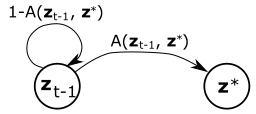
\includegraphics[width=6cm]{mcmc_accept.png}
\caption{Transition from $\bm{z}_{t-1}$ to $\bm{z}_t$}
\label{fig:mcmc_accept}
\end{figure}
\subsection{Construction and Interpretation of the Transition Probability $T\left(\bm{z}_{t}|\bm{z}_{t-1}\right)$}
The transition probability is expressed as follows.
\begin{equation}
\begin{aligned}
T\left(\bm{z}_{t}|\bm{z}_{t-1}\right)
&= q\left(\bm{z}_{t}|\bm{z}_{t-1}\right)A\left(\bm{z}_{t-1}, \bm{z}_{t}\right)\\
&\:\:\:\:+ \delta_{\bm{z}_{t-1}}\left(\bm{z}_{t}\right)
\int q\left(\bm{z}^*|\bm{z}_{t-1}\right)\left(1 - A\left(\bm{z}_{t-1}, \bm{z}^*\right)\right)d\bm{z}^*
\label{eq:definition_T}\\
\end{aligned}
\end{equation}
This is difficult to grasp but it can be explained as follows.
First, we show the validity of $\int T\left(\bm{z}_{t}|\bm{z}_{t-1}\right)$.
\begin{equation}
\begin{aligned}
\int T\left(\bm{z}_{t}|\bm{z}_{t-1}\right)d\bm{z}_t
&= \int q\left(\bm{z}_{t}|\bm{z}_{t-1}\right)A\left(\bm{z}_{t-1}, \bm{z}_{t}\right)d\bm{z}_t\\
&\:\:\:\:+ \int \delta_{\bm{z}_{t-1}}\left(\bm{z}_{t}\right)
\left(\int q\left(\bm{z}^*|\bm{z}_{t-1}\right)\left(1 - A\left(\bm{z}_{t-1}, \bm{z}^*\right)\right)d\bm{z}^*\right) d\bm{z}_t\\
&= \int q\left(\bm{z}_{t}|\bm{z}_{t-1}\right)A\left(\bm{z}_{t-1}, \bm{z}_{t}\right)d\bm{z}_t\\
&\:\:\:\:+ \int q\left(\bm{z}^*|\bm{z}_{t-1}\right)\left(1 - A\left(\bm{z}_{t-1}, \bm{z}^*\right)\right)d\bm{z}^*\\
&= \int q\left(\bm{z}|\bm{z}_{t-1}\right)A\left(\bm{z}_{t-1}, \bm{z}\right)d\bm{z}
+ \int q\left(\bm{z}|\bm{z}_{t-1}\right)\left(1 - A\left(\bm{z}_{t-1}, \bm{z}\right)\right)d\bm{z}\\
&= \int q\left(\bm{z}|\bm{z}_{t-1}\right)d\bm{z} = 1\\
\end{aligned}
\end{equation}
Also, it is easy to see that $T\left(\bm{z}_{t}|\bm{z}_{t-1}\right) \ge 0$ for any $\bm{z}_t$ in the domain.
Therefore $T\left(\bm{z}_{t}|\bm{z}_{t-1}\right)$ is a valid probability density function.


Next, we interpret $\int T\left(\bm{z}_{t}|\bm{z}_{t-1}\right)$, for that we take an integral of
$T\left(\bm{z}_{t}|\bm{z}_{t-1}\right)$ for an infinitesimal region $\Delta\bm{z}$.
If $\bm{z}_{t-1} \notin \Delta\bm{z}$, then
\begin{equation}
\begin{aligned}
\int_{\Delta\bm{z}} T\left(\bm{z}_{t}|\bm{z}_{t-1}\right)d\bm{z}_t
&= \int_{\Delta\bm{z}} q\left(\bm{z}_{t}|\bm{z}_{t-1}\right)A\left(\bm{z}_{t-1}, \bm{z}_{t}\right)d\bm{z}_t\\
\end{aligned}
\end{equation}
This means the probability of transition to the new region specified by $\Delta\bm{z}$ which is represented by $\bm{z}_t$.
On the other hand, if $\bm{z}_{t-1} \in \Delta\bm{z}$, then
\begin{equation}
\begin{aligned}
\int_{\Delta\bm{z}} T\left(\bm{z}_{t}|\bm{z}_{t-1}\right)d\bm{z}_t
&= \int_{\Delta\bm{z}} q\left(\bm{z}_{t}|\bm{z}_{t-1}\right)A\left(\bm{z}_{t-1}, \bm{z}_{t}\right)d\bm{z}_t\\
&\:\:\:\:+ \int q\left(\bm{z}^*|\bm{z}_{t-1}\right)\left(1 - A\left(\bm{z}_{t-1}, \bm{z}^*\right)\right)d\bm{z}^*\\
&= \int_{\Delta\bm{z}} q\left(\bm{z}|\bm{z}_{t-1}\right) A\left(\bm{z}_{t-1}, \bm{z}\right)d\bm{z}\\
&\:\:\:\:+ \int q\left(\bm{z}|\bm{z}_{t-1}\right)d\bm{z}
- \int q\left(\bm{z}|\bm{z}_{t-1}\right) A\left(\bm{z}_{t-1}, \bm{z}\right)d\bm{z}\\
&= \int q\left(\bm{z}|\bm{z}_{t-1}\right)d\bm{z}
- \int_{\setminus\Delta\bm{z}} q\left(\bm{z}|\bm{z}_{t-1}\right) A\left(\bm{z}_{t-1}, \bm{z}\right)d\bm{z}\\
&= \int_{\Delta\bm{z}} q\left(\bm{z}|\bm{z}_{t-1}\right)d\bm{z}
+ \int_{\setminus\Delta\bm{z}} q\left(\bm{z}|\bm{z}_{t-1}\right)\left(1 - A\left(\bm{z}_{t-1}, \bm{z}\right)\right)d\bm{z}\label{eq:mcmc_T}\\
\end{aligned}
\end{equation}
where $\setminus\Delta\bm{z}$ means the domain of $\bm{z}$ excluding $\Delta\bm{z}$.
The first term of equation \ref{eq:mcmc_T} means the probability of staying in the region represented by $\bm{z}_{t-1}$.
The second term means the probability of trying to transit to another region but rejected, and eventually staying in the
current region represented by $\bm{z}_{t-1}$.


\subsection{How to Find an Ergodic $T\left(\bm{z}_{t}|\bm{z}_{t-1}\right)$?}
We want to find $T\left(\bm{z}_{t}|\bm{z}_{t-1}\right)$ such that
$T\left(\bm{z}_{t}|\bm{z}_{t-1}\right)= p(\bm{z}_{t})$ as $t \rightarrow \infty$ for any $\bm{z}_0$.
This is achieved if $T\left(\bm{z}_{t}|\bm{z}_{t-1}\right)= p(\bm{z}_{t})$ is ergodic, and a sufficient
condition for the ergodicity is called \textit{detailed balance},
for which equation \ref{eq:detailed_balance} must hold for any $\bm{z}_{a}$, and $\bm{z}_{b}$.
\begin{equation}
\begin{aligned}
p(\bm{z}_b) T(\bm{z}_{a}|\bm{z}_{b}) = p(\bm{z}_a) T(\bm{z}_{b}|\bm{z}_{a})\label{eq:detailed_balance}
\end{aligned}
\end{equation}

It has the following invariant property.
\begin{equation}
\begin{aligned}
\int p(\bm{z}_a) T(\bm{z}_{b}|\bm{z}_{a}) d\bm{z}_a
&= \int p(\bm{z}_b) T(\bm{z}_{a}|\bm{z}_{b}) d\bm{z}_a\\
&= p(\bm{z}_b) \int T(\bm{z}_{a}|\bm{z}_{b}) d\bm{z}_a\\
&= p(\bm{z}_b)\\
\end{aligned}
\end{equation}

Hatings\cite{mcmc_hastings} found in 1970 one such $A\left(\bm{z}_{t-1}, \bm{z}_{t}\right)$, which satisfies detailed balance.
\begin{equation}
\begin{aligned}
A\left(\bm{z}_{t-1}, \bm{z}_{t}\right)
 = \min\left\{1, \frac{p(\bm{z}_t)q(\bm{z}_{t-1}|\bm{z}_t)}{p(\bm{z}_{t-1})q(\bm{z}_{t}|\bm{z}_{t-1})}\right\}
\label{eq:metropolis_hastings}
\end{aligned}
\end{equation}
Please note that we can use unnormalized probability density functions as follows.
\begin{equation}
\begin{aligned}
A\left(\bm{z}_{t-1}, \bm{z}_{t}\right)
 = \min\left\{1, \frac{\tilde{p}(\bm{z}_t)q(\bm{z}_{t-1}|\bm{z}_t)}{\tilde{p}(\bm{z}_{t-1})q(\bm{z}_{t}|\bm{z}_{t-1})}\right\}
\end{aligned}
\end{equation}



Following shows that the acceptance function in equation \ref{eq:metropolis_hastings} meets the detailed balance.
If $\bm{z}_{t-1} = \bm{z}_t$, then it trivially holds.
If $\bm{z}_{t-1} \ne \bm{z}_t$, then,
\begin{equation}
\begin{aligned}
p(\bm{z}_{t-1})T(\bm{z}_{t}|\bm{z}_{t-1}) &= p(\bm{z}_{t-1})q(\bm{z}_{t}|\bm{z}_{t-1})A(\bm{z}_{t-1}, \bm{z}_{t})
\:\:\:\:\text{(from equation \ref{eq:definition_T})}\\
&= \min\left\{\:p(\bm{z}_{t-1})q(\bm{z}_{t}|\bm{z}_{t-1}),\:\: p(\bm{z}_{t})q(\bm{z}_{t-1}|\bm{z}_{t})\:\right\}\\
&= \min\left\{\:p(\bm{z}_{t})q(\bm{z}_{t-1}|\bm{z}_{t}),\:\: p(\bm{z}_{t-1})q(\bm{z}_{t}|\bm{z}_{t-1})\:\right\}\\
&= p(\bm{z}_{t})q(\bm{z}_{t-1}|\bm{z}_{t})A(\bm{z}_{t}, \bm{z}_{t-1})\\
&= p(\bm{z}_{t})T(\bm{z}_{t-1}|\bm{z}_{t})\\
\end{aligned}
\end{equation}

This is called \textit{Metropolis-Hastings} algorithm. Usually a multivariabe normal distribution, whose mean
is $\bm{z}_{t-1}$, is used as a proposal distribution $q(\bm{z}_{t}|\bm{z}_{t-1})$.
The drawback of using this proposal distribution is that $\bm{z}_0, \bm{z}_1, \cdots$ becomes a random walk, and
the distance is in the order of $\sqrt{t}$.

\section{Gibbs Sampling}
This is a MCMC with a particular proposal distribution,
in which one element $z^i$ of $\bm{z} = (z^1, z^2, \cdots, z^N)$ is conditioned on the rest $\bm{z}^{\setminus i}$,
such that $q(z^i_{t}) = p(z^i_{t}|\bm{z}^{\setminus i}_{t-1})$
In this case, the transition is always accepted as the following acceptance probability function 
implies.

\begin{equation}
\begin{aligned}
A\left(\bm{z}_{t-1}, \bm{z}_{t}\right)
 &= \min\left\{1, 
                \frac{ p(\bm{z}_t)q(\bm{z}_{t-1}|\bm{z}_t) }
                     { p(\bm{z}_{t-1})q(\bm{z}_{t}|\bm{z}_{t-1}) }
    \right\}\\
 &= \min\left\{1,
                \frac{ p(\bm{z}_t)     p(z^i_{t-1} |\bm{z}^{\setminus i}_t)     }
                     { p(\bm{z}_{t-1}) p(z^i_{t}   |\bm{z}^{\setminus i}_{t-1}) }
    \right\}\\
 &= \min\left\{1,
                \frac{ p(z^i_{t},   \bm{z}^{\setminus i}_{t})   p(z^i_{t-1}|\bm{z}^{\setminus i}_t    ) }
                     { p(z^i_{t-1}, \bm{z}^{\setminus i}_{t-1}) p(z^i_{t}  |\bm{z}^{\setminus i}_{t-1}) }
    \right\}\\
 &= \min\left\{1,
             \frac{ p(z^i_{t}   |\bm{z}^{\setminus i}_{t}  ) p(\bm{z}^{\setminus i}_{t})   p(z^i_{t-1}|\bm{z}^{\setminus i}_t    ) }
                  { p(z^i_{t-1} |\bm{z}^{\setminus i}_{t-1}) p(\bm{z}^{\setminus i}_{t-1}) p(z^i_{t}  |\bm{z}^{\setminus i}_{t-1}) }
    \right\}\\
 &= \min\left\{1,
             \frac{ p(z^i_{t}   |\bm{z}^{\setminus i}_{t-1}) p(\bm{z}^{\setminus i}_{t-1}) p(z^i_{t-1}|\bm{z}^{\setminus i}_{t-1}) }
                  { p(z^i_{t-1} |\bm{z}^{\setminus i}_{t-1}) p(\bm{z}^{\setminus i}_{t-1}) p(z^i_{t}  |\bm{z}^{\setminus i}_{t-1}) }
    \right\}\:\:\:\:\:\:\left(\bm{z}^{\setminus i}_{t} = \bm{z}^{\setminus i}_{t-1} \right)\\
 &= \min\left\{1,1\right\} = 1\label{eq:gibbs}\\
\end{aligned}
\end{equation}

The index $i$ for the element $z^i$ is cyclically iterated or randomly chosen.


\section{MCMC with Hamiltonian dynamics}
Here the emphasis is on the regorous formation of MCMC using Hamiltonian proposal distribution, as
almost all the books and articles focus on the Hamiltonian dynamics and numerical integration.
11.5 of PRML \cite{bishop2007}, which gives a good overview.
For deeper understanding, read the chapter on handbook by Neal \cite{hmcmc_neal}, which is freely available online.
It is also useful to read section 3 ``The foundations of Hamiltonian Monte Carlo''  and 4 ``Efficient Hamiltonion Monte Carlo''
of the article by Betancourt \cite{hmcmc_betancourt}.
All the articles and books I have read put emphasis on Hamiltonian dynamics and its numerical integration,
but more rigorous formation of MCMC using Hamiltonian dynamics is often neglected.
Especially, formation of a proposal function, an acceptance function, transition probability distribution and ergodicity
are not well discussed. This section focus on those topics, rather than the Hamiltonion dynamics
and the numerical simulation, as I'm already well versed with physics simulation.

This is an attempt to overcome the limited travel of random walk by drawing a sample from an ordinary proposal distribution $q(\bm{z})$.
The basic idea is to introduce a new variable (kind of latent variable) $\bm{r}$ and to form a joint distribution 
$p(\bm{z}, \bm{r}) = p_{model}(\bm{z}) q(\bm{r})$. $q(\bm{r})$ is a multivariate Gaussian distribution, which is also considered a
negative of kinetic energy in Hamiltonian dynamics.
At each step, we have a previously drawn sample $(\bm{z}_i, \bm{r}_i)$.
First we draw a sample $\bm{r}_i^*$ from $q(\bm{r})$, and then we deterministically find the next sample 
$(\bm{z}_{i+1}, \bm{r}_{i+1})$ from $(\bm{z}_{i}, \bm{r}_{i}^*)$ such that 
$p(\bm{z}_{i+1}, \bm{r}_{i+1}) = p(\bm{z}_{i}, \bm{r}_{i}^*)$, hoping $\bm{z}_{i+1}$ has travelled further from $\bm{z}_i$
using Hamiltonian dynamics.
The first part is considered Gibbs sampling, and hence the detailed balance holds.
The second deterministic part is carefully designed to hold the detailed balance.
However, due to the determinism, neither irreducibility or aperiodicity holds.
Hence the ergodicity of the whole process must be proven separately.


\subsection{Augmentation of the model distribution $p_{model}(\bm{z})$ with momentum $\bm{r}$}
Given a distribution $p_{model}(\bm{z})$, $\bm{z} \in \mathcal{R}^d$,  from which you want to draw samples, we augment
it with an additional variable $\bm{r}$, $\bm{r} \in \mathcal{R}^d$, which works as a momemtum. The joint distribution of $\bm{z}$ and
$\bm{r}$ is defined as follows.

\begin{equation}
\begin{aligned}
p(\bm{z}, \bm{r}) = p_{model}(\bm{z})\:p_{\bm{r}}(\bm{r})
\end{aligned}
\end{equation}
where $p_{\bm{r}}(\bm{r})$ is a Gaussian distribution with zero mean as follows.
\begin{equation}
\begin{aligned}
p_{\bm{r}}(\bm{r}) = \frac{1}{Z_{\bm{r}}} \exp \left( -\frac{1}{2}\bm{r}^T M^{-1}\bm{r}\right)
\end{aligned}
\end{equation}
where $M$ is a diagonal mass matrix.
The original distribution $p_{model}(\bm{z})$ corresponds to a potential energy.
\begin{equation}
\begin{aligned}
U(\bm{z}) = -\ln\left(p_{model}(\bm{z})\right)
\end{aligned}
\end{equation}
And the kinetic energy is defined as follows.
\begin{equation}
\begin{aligned}
K(\bm{r}) \propto -\ln\left(p_{\bm{r}}(\bm{r})\right)= -\frac{1}{2}\bm{r}^T M^{-1}\bm{r}
\end{aligned}
\end{equation}
In the simplest form $K(\bm{r}) = \frac{1}{2} \sum_{i=1}^{d}r_i^2$, and $\bm{r}$ works as velocity.
Finally the Hamiltonian is defined as follows.
\begin{equation}
\begin{aligned}
H(\bm{z}, \bm{r}) &= U(\bm{z}) + K(\bm{r})
\end{aligned}
\end{equation}
The motion dynamics of $\bm{z}$ and $\bm{r}$ over continuous time $t$ is as follows.
\begin{equation}
\begin{aligned}
\frac{dz_i}{dt} &= \frac{{\partial}H}{\partial r_i}  = \left[M^{-1}\bm{r}\right]_i\label{eq:dynamics_1}\\
\end{aligned}
\end{equation}
\begin{equation}
\begin{aligned}
\frac{dr_i}{dt} &= -\frac{{\partial}H}{\partial z_i} = 
-\frac{{\partial}U}{\partial z_i}\label{eq:dynamics_2}\\
\end{aligned}
\end{equation}
From the equations \ref{eq:dynamics_1} \& \ref{eq:dynamics_2}, we can determine
$\left(\bm{z}(t_0 + {\Delta}t), \bm{r}(t_0 + {\Delta}t)\right)$ from 
$\left(\bm{z}(t_0), \bm{r}(t_0)\right)$ and ${\Delta}t$, considering $\bm{z}$ and $\bm{r}$ functions of $t$.
We use three laws regarding the Hamiltonian motion dynamics.


\subsubsection{Reversibility of Motion}
This means we can find $\left(\bm{z}(t_0), \bm{r}(t_0)\right)$ from
$\left(\bm{z}(t_0 + {\Delta}t), \bm{r}(t_0 + {\Delta}t)\right)$ and $-{\Delta}t$.

\subsubsection{Conservation of Energy}
This means 
$H\left(\bm{z}(t_0 + {\Delta}t), \bm{r}(t_0 + {\Delta}t)\right) = H\left(\bm{z}(t_0), \bm{r}(t_0)\right)$
This is proven as follows.
\begin{equation}
\begin{aligned}
\frac{dH}{dt}
&= \sum_{i=1}^d\left[\frac{dz_i}{dt}\frac{{\partial}H}{{\partial}z_i} + \frac{dr_i}{dt}\frac{{\partial}H}{{\partial}r_i}\right]\\
&= \sum_{i=1}^d\left[ \frac{{\partial}H}{{\partial}r_i}\frac{{\partial}H}{{\partial}z_i}
                        - \frac{{\partial}H}{{\partial}z_i}\frac{{\partial}H}{{\partial}r_i} \right] = 0\\
\end{aligned}
\end{equation}

\subsubsection{Conservation of Volume}
Let $R(t_0) \subset \mathcal{R}^{2d}$ be a closed bounded volume whose points represent $(\bm{z}, \bm{r})$,
and $R(t_0 + {\Delta}t)$ be the same volume at time $t + {\Delta}t$.
Then $||R(t_0)|| = ||R(t_0 + {\Delta}t)||$.
This is comes from something called Liouville's Theorem for symplectic geometry.
Most of the MCMC articles and books skip the proof.
The cleanest and clearest explanation for the proof that I know is given in the physics book by Arnold\cite{arnold_1989},
Chap. 15 \textit{Hamilton's equations}, and Chap 16 \textit{Liouville's theorem}.
Following gives an outline.

Let the $2d$-dimensional space determined by $\bm{z}, \bm{r}$ denoted by \textit{phrase space}.
Let the group of transformations over time ${\Delta}t$ from $t_0$ denoted by
\textit{phase flow}.
$$ g^{{\Delta}t}: 
(\bm{z}(t_0), \bm{r}(t_0)) \mapsto 
(\bm{z}(t_0 + {\Delta}t), \bm{r}(t_0 + {\Delta}t))$$

\cite{arnold_1989} leaves the proof that $\{g^{{\Delta}t}\}$ forms a group, but
basically we need to provide the following
\begin{itemize}
\item Closure for addition:  Addition of two phase flows is another phase flow.
\item Associativity: $(g^{{\Delta}t_a} + g^{{\Delta}t_b}) +  g^{{\Delta}t_c} = 
        g^{{\Delta}t_a} +  (g^{{\Delta}t_b} +  g^{{\Delta}t_c})$
\item Identity element: $g^{{\Delta}t_0}$ is a flow such that
$$ (\bm{z}(t_0), \bm{r}(t_0)) = (\bm{z}(t_0 + {\Delta}t), \bm{r}(t_0 + {\Delta}t))$$
\item Inverse element: For each $g^{{\Delta}t_0}$ there is an inverse flow
such that
$$ -g^{{\Delta}t}: (\bm{z}(t_0), \bm{r}(t_0)) \mapsto 
(\bm{z}(t_0 - {\Delta}t), \bm{r}(t_0 - {\Delta}t))$$
\end{itemize}

Let $(\dot{\bm{z}}, \dot{\bm{r}}) = \bm{f}(\bm{z}, \bm{r})$ be the ODE of
Hamiltonian dynamics such that
\begin{equation}
\bm{f}(\bm{z}, \bm{r}) = \left[
\begin{array}{c}
    \frac{\partial H}{\partial \bm{r} }\\
    \hline
    - \frac{\partial H}{\partial \bm{z} }
    \end{array}\right]\label{eq:hmc_def_f}
\end{equation}


Then the phase flow is approximated as follows.

\begin{equation}
\begin{aligned}
g^{{\Delta}t}(\bm{z}(t_0), \bm{r}(t_0)) = (\bm{z}(t_0), \bm{r}(t_0)) + \bm{f}(\bm{z}, \bm{r})|_{\bm{z}(t_0),\bm{r}(t_0)}{\Delta}t + O({\Delta}t^2)\label{eq:hamiltonioan_ode}\\
\end{aligned}
\end{equation}

Then we can express the volumes as folows.
\begin{equation}
\begin{aligned}
R(t_0 + {\Delta}t) = g^{{\Delta}t_a}( R(t_0) )
\end{aligned}
\end{equation}

Then the formula for changing variables in a multiple integral gives.
(
$(\bm{z}(t_0), \bm{r}(t_0)) \mapsto 
(\bm{z}(t_0 + {\Delta}t), \bm{r}(t_0 + {\Delta}t))$ can be considered
a change in the variables.)

\begin{equation}
\begin{aligned}
|R(t_0 + {\Delta}t)| = 
\int_{R(t_0)}
    \det
    \left( \frac{ \partial g^{{\Delta}t}(\bm{z}(t_0), \bm{r}(t_0)) }
                { \partial (\bm{z}(t_0) ,\bm{r}(t_0)) }
    \right)
\partial(\bm{z}(t_0)\bm{r}(t_0))\label{eq:hmc_volume_R_t1_deltat}
\end{aligned}
\end{equation}

From equation \ref{eq:hamiltonioan_ode},
\begin{equation}
\begin{aligned}
\frac{ \partial g^{{\Delta}t}(\bm{z}(t_0), \bm{r}(t_0))}
     { \partial (\bm{z}(t_0) \bm{r}(t_0)) }
 = I_{2d} + 
\frac{\partial \bm{f}}{\partial(\bm{z}(t_0), \bm{r}(t_0))}{\Delta}t
+ O({\Delta}t^2)
\end{aligned}
\end{equation}

Then
\begin{equation}
\begin{aligned}
\det\left(\frac{ \partial g^{{\Delta}t}(\bm{z}(t_0), \bm{r}(t_0))}
     { \partial (\bm{z}(t_0) \bm{r}(t_0)) }\right)
 &= 1 + \text{tr} \left( \frac{ \partial \bm{f} }
                       { \partial(\bm{z}(t_0), \bm{r}(t_0)) }
           \right){\Delta}t
+ O({\Delta}t^2)\\
 &= 1 + \div \bm{f}{\Delta}t + O({\Delta}t^2)\label{eq:hmc_det_div}
\end{aligned}
\end{equation}

And the divergence is zero as follows. From equation \ref{eq:hmc_def_f},
\begin{equation}
\begin{aligned}
\div\bm{f} = \frac{\partial}
                  {\partial{\bm{z}} }
             \frac{\partial H}
                  {\partial \bm{r} }
           - \frac{\partial}{\partial{\bm{r}}}
             \frac{\partial H}{\partial \bm{z} } = 0\label{eq:hmc_div_0}
\end{aligned}
\end{equation}

From equations \ref{eq:hmc_det_div} \& \ref{eq:hmc_div_0},
\begin{equation}
\begin{aligned}
\det\left(\frac{ \partial g^{{\Delta}t}(\bm{z}(t_0), \bm{r}(t_0))}
     { \partial (\bm{z}(t_0) \bm{r}(t_0)) }\right)
 &= 1 + O({\Delta}t^2)\label{eq:hmc_det_div_simplified}
\end{aligned}
\end{equation}

From equations \ref{eq:hmc_volume_R_t1_deltat} 
and \ref{eq:hmc_det_div_simplified},

\begin{equation}
\begin{aligned}
\frac{d|R(t_0 + {\Delta}t)|}
     {d{\Delta}t}
&= 
\frac{d}{d{\Delta}t}
\int_{R(t_0)}
    \left(1 + O({\Delta}t^2)\right)\:
\partial(\bm{z}(t_0)\bm{r}(t_0))\\
&= 
\int_{R(t_0)}
\frac{d}{d{\Delta}t}
    \left(1 + O({\Delta}t^2)\right)\:
\partial(\bm{z}(t_0)\bm{r}(t_0))\\
&= 0
\end{aligned}
\end{equation}

Hence $|R(t_0 + {\Delta}t)| = |R(t_0)|$,
and the convervation of the volume holds.

The volume preservation and reversibility over time implies that 
the phase flow is a bijection (one-to-one mapping).

\subsection{Hamiltonian Dynamics for a Step}
This is a numerical integration of phase flow ODE over time $t$ defined
in equations \ref{eq:hmc_def_f} \& \ref{eq:hamiltonioan_ode}.
It seems an Euler variant called the leap frog method is used as follows.
\begin{equation}
\begin{aligned}
r_i(t + \epsilon/2) 
&= r_i(t) - (\epsilon/2)\frac{\partial U}{\partial z_i}z_i(t)\\
z_i(t+\epsilon) &= z_i(t) + \epsilon\frac{r_i(t+\epsilon/2)}{m_i}\\
r_i(t + \epsilon)
&= r_i(t + \epsilon/2) - 
   (\epsilon/2)\frac{\partial U}{\partial z_i}z_i(t+\epsilon)\\
\end{aligned}
\end{equation}
It is an explicit method, 
but neither  $U(\bm{z})$ or $K(\bm{r})$ is steep enough to cause stiffness.

One step $(\bm{z}_{i+1}, \bm{r}_{i+1}) = \phi(\bm{z}_i, \bm{r}_i)$ consists of $L$ numerical integration of time step $\epsilon$.
There is one tweek to make the step symmetry. At the last step, we flip the
sign of each $r_i$ so that the following also holds.
$(\bm{z}_{i}, \bm{r}_{i}) = \phi(\bm{z}_{i+1}, \bm{r}_{i+1})$.
Flipping of the sing of  $r_i$ has the same effect as numerical integration
over negative time $-\epsilon$ toward past.

\subsection{Proposal Distribution}

The hamitonian dynamics at one step is given as follows.
$(\bm{z}_{i+1}, \bm{r}_{i+1})= \bm{\phi}(\bm{z}_{i}, \bm{r}_{i})$.
This is a symmetric process as in
$(\bm{z}_{i}, \bm{r}_{i})= \bm{\phi}(\bm{z}_{i+1}, \bm{r}_{i+1})$.
This is achieved by flipping the polarity of $\bm{r}$ after the numerical integration finished as stated in the previous section..

The proposal distribution is a deterministic process whose density function is given as follows.

\begin{equation}
\begin{aligned}
q(\bm{z}, \bm{r}|\bm{z}_i, \bm{r}_i) = 
\delta\left(\bm{z} - \bm{\phi}(\bm{z}_i)\right)\delta\left(\bm{r} - \bm{\phi}(\bm{r}_i)\right)
\end{aligned}
\end{equation}

Please note that $q(\bm{z}, \bm{r}|\bm{z}_i, \bm{r}_i)$ is everywehere 0 except for 
$(\bm{\phi}(\bm{z}_i), \bm{\phi}(\bm{r}_i))$. This means the detailed balance of the transition
probability $T(\bm{z},\bm{r}|\bm{z}_i, \bm{r}_i)$ is not enouch to prove the ergodicity.
This will be discussed later.

\subsection{Acceptance Function}
The acceptance function must be defined on volume, not on point.
For that, we extend the hamiltonian dynamics function from the point to volume as follows.
Let ${\partial}R \subseteq \mathcal{R}^{2d}$ be a closed bounded volume
defined in $(\bm{z},\bm{r})$ phase space.
Let ${\partial}R_{i+1}= \bm{\phi}({\partial}R_{i})$
The symmetry still holds.
${\partial}R_{i} = \bm{\phi}({\partial}R_{i+1})$

The acceptance probability is defined as follows, provided $|{\partial}R_a| = |{\partial}R_b|$.
\begin{equation}
\begin{aligned}
A({\partial}R_a, {\partial}R_b) = 
    \begin{cases}
        {p(\bm{z}_b, \bm{r}_b)}/{p(\bm{z}_a, \bm{r}_a)} & {\partial}R_b = \bm{\phi}({\partial}R_a)\\
        \text{undefined} & \text{otherwise}\\
    \end{cases}\label{eq:hmc_acceptance}
\end{aligned}
\end{equation}
where $(\bm{z}_a, \bm{r}_a) \in {\partial}R_a$, and
$(\bm{z}_b, \bm{r}_b) = \bm{\phi}(\bm{z}_a, \bm{r}_a) \in {\partial}R_b$,
and we assume $p(\bm{z}, \bm{r})$ is constant in a minute volume ${\partial}R$.

The following derives equation \ref{eq:hmc_acceptance}.
First, we form the Metropolis acceptance from its definition.
\begin{equation}
\begin{aligned}
A({\partial}R_a, {\partial}R_b) = \min \left\{
1,
\frac{
    \int_{{\partial}R_a} \int_{{\partial}R_b}
        p( \bm{z}_b, \bm{r}_b ) q( \bm{z}_a, \bm{r}_a | \bm{z}_b, \bm{r}_b )
    \partial(\bm{z}_b\bm{r}_b) \partial(\bm{z}_a\bm{r}_a)
}
{
    \int_{{\partial}R_b} \int_{{\partial}R_a}
        p( \bm{z}_a, \bm{r}_a ) q( \bm{z}_b, \bm{r}_b | \bm{z}_a, \bm{r}_a )
    \partial(\bm{z}_a\bm{r}_a) \partial(\bm{z}_b\bm{r}_b)
}
\right\}
\end{aligned}
\end{equation}

The numerator of the second term in the $\min$ is expanded into:
\begin{equation}
\begin{aligned}
\text{term1} &=
    \int_{{\partial}R_a} \int_{{\partial}R_b}
        p( \bm{z}_b, \bm{r}_b )
        \delta\left(\bm{z}_a - \bm{\phi}(\bm{z}_b)\right)
        \delta\left(\bm{r}_a - \bm{\phi}(\bm{r}_b)\right)
    \partial(\bm{z}_b\bm{r}_b) \partial(\bm{z}_a\bm{r}_a)\\
&=
    \int_{{\partial}R_b}
        p( \bm{z}_b, \bm{r}_b )
    \int_{{\partial}R_a} 
        \delta\left(\bm{z}_a - \bm{\phi}(\bm{z}_b)\right)
        \delta\left(\bm{r}_a - \bm{\phi}(\bm{r}_b)\right)
    \partial(\bm{z}_a\bm{r}_a)
    \partial(\bm{z}_b\bm{r}_b)\\
&=
    \begin{cases}
        0 & {\partial}R_b \cap \bm{\phi}({\partial}R_a) = \emptyset\\
        \int_{{\partial}R_b}p( \bm{z}_b, \bm{r}_b )\partial(\bm{z}_b\bm{r}_b)
        & {\partial}R_b = \bm{\phi}({\partial}R_a)\\
    \end{cases}\\
&=
    \begin{cases}
        0 & {\partial}R_b \cap \bm{\phi}({\partial}R_a) = \emptyset\\
        \left|{\partial}R_a\right|p( \bm{z}_b, \bm{r}_b )
        & {\partial}R_b = \bm{\phi}({\partial}R_a)\\
    \end{cases}
\end{aligned}
\end{equation}


In the same way, the denominator of the second term in the $\min$ is expanded into:
\begin{equation}
\begin{aligned}
\text{term2} &=
    \begin{cases}
        0 & {\partial}R_b \cap \bm{\phi}({\partial}R_b) = \emptyset\\
        \left|{\partial}R_b\right|p( \bm{z}_a, \bm{r}_a )
        & {\partial}R_a = \bm{\phi}({\partial}R_b)\\
    \end{cases}
\end{aligned}
\end{equation}
Because of the conservation of the volume and the reversibility of $\phi$, 
$$ {\partial}R_a = \bm{\phi}({\partial}R_b) \Leftrightarrow
 {\partial}R_b = \bm{\phi}({\partial}R_a)$$

Due to the determinism of $phi$, the undefined case in equation 
\ref{eq:hmc_acceptance} never occurs.
Also, due to conservation of energy, the first case in equations
\ref{eq:hmc_acceptance} \& \ref{eq:hmc_acceptance2} is theoretically $1$,
but it can be slightly different due to numerical error in the integration.


\subsection{Transition Probability and Detailed Balance}
The transition probability is defined in equation \ref{eq:definition_T}.
We restate it as follows.
\begin{equation}
\begin{aligned}
T\left(\bm{z}_{t}|\bm{z}_{t-1}\right)
&= q\left(\bm{z}_{t}|\bm{z}_{t-1}\right)A\left(\bm{z}_{t-1}, \bm{z}_{t}\right)\\
&\:\:\:\:+ \delta\left(\bm{z}_{t} - \bm{z}_{t-1}\right)
\int q\left(\bm{z}^*|\bm{z}_{t-1}\right)\left(1 - A\left(\bm{z}_{t-1}, \bm{z}^*\right)\right)d\bm{z}^*
\end{aligned}
\end{equation}
The first term indicates the probability in which the proposed $\bm{z}_t$
was accepted. The second term indicates 
the collective probability in which the proposed $\bm{z}^*$ was rejected,
and it has to stay in $\bm{z}_{t-1}$.

However, in the case of Hamiltonian transition, there is only one deterministic
transition and it is simplified as follows.
\begin{equation}
\begin{aligned}
T\left(\bm{z}_{i+1}, \bm{r}_{i+1}|\bm{z}_{i}, \bm{r}_{i}\right) = 
    \begin{cases}
        \min \left\{ 1,
            \frac{ p( \bm{\phi}(\bm{z}_i), \bm{\phi}(\bm{r}_i) ) }
                 { p( \bm{z}_i, \bm{r}_i ) } \right\}
 & \bm{z}_{i+1} = \bm{\phi}(\bm{z}_i) \wedge
   \bm{r}_{i+1} = \bm{\phi}(\bm{r}_i)\\
        1 - \min \left\{ 1,
            \frac{ p( \bm{\phi}(\bm{z}_i), \bm{\phi}(\bm{r}_i) ) }
                 { p( \bm{z}_i, \bm{r}_i ) } \right\}
 & \bm{z}_{i+1} = \bm{z}_i \wedge \bm{r}_{i+1} = \bm{r}_i\\
        0 & \text{otherwise}
    \end{cases}
\end{aligned}
\end{equation}

The detailed balance holds as follows.
First, if  $\bm{z}_{i+1} = \bm{\phi}(\bm{z}_i) \wedge 
     \bm{r}_{i+1} = \bm{\phi}(\bm{r}_i)$, then from the symmetry of $\phi$,
$\bm{z}_{i} = \bm{\phi}(\bm{z}_{i+1}) \wedge 
 \bm{r}_{i} = \bm{\phi}(\bm{r}_{i+1})$, and
\begin{equation}
\begin{aligned}
    p\left(\bm{z}_i, \bm{r}_i\right)
    T\left(\bm{z}_{i+1}, \bm{r}_{i+1}|\bm{z}_{i}, \bm{r}_{i}\right)
&= 
    \min \left\{
           p( \bm{z}_i, \bm{r}_i ),
           p( \bm{\phi}(\bm{z}_i), \bm{\phi}(\bm{r}_i) )
          \right\}\\
&= 
    \min \left\{
           p( \bm{\phi}(\bm{z}_{i+1}), \bm{\phi}(\bm{r}_{i+1}) ),
           p( \bm{z}_{i+1}, \bm{r}_{i+1} )
          \right\}\\
&=
    p\left(\bm{z}_{i+1}, \bm{r}_{i+1}\right)
    T\left(\bm{z}_{i}, \bm{r}_{i}|\bm{z}_{i+1}, \bm{r}_{i+1}\right)
\end{aligned}
\end{equation}
So the it holds.
Second, if $\bm{z}_{i+1} = \bm{z}_i \wedge \bm{r}_{i+1} = \bm{r}_i$, then
the it holds.
Otherwise,
$T\left(\bm{z}_{i+1}, \bm{r}_{i+1}|\bm{z}_{i}, \bm{r}_{i}\right) = 0$, and
it trivially holds.

\subsection{Additional Gibb Sampling per Step and Ergodicity}
The Hamiltonian step described above itself does not ensure ergodicity.
In fact, without additional step, it oscillates between 
$( \bm{z}_{i}, \bm{r}_{i} )$ and $(\bm{z}_{i+1}, \bm{r}_{i+1})$ due
to the symmetry of $\phi$. For ergodicity, we draw a fresh $\bm{r}$
before each Hamiltonian step. So, one step to draw a sample consists of
the following.
\begin{itemize}
\item Before the step, we have $( \bm{z}_{i-1}, \bm{r}_{i-1} )$, and 
corresponding energy $H_{i-1} = U(\bm{z}_{i-1}) + K(\bm{r}_{i-1} )$.
\item Draw
$\bm{r}^*_{i-1} \sim \mathcal{N}\left( \bm{r}^*_{i-1};0, M^{-1}\right)$.
Energy changes to $H^*_{i-1} = U(\bm{z}_{i-1}) + K(\bm{r}^*_{i-1} )$.
\item Make transition to
$(\bm{z}_{i}, \bm{r}_{i}) = 
\left( \bm{\phi}(\bm{z}_{i-1}), \bm{\phi}(\bm{r}^*_{i-1}) \right)$ if
it is accepted. The energy does not change theorecitally, but might change
due to numerical error.
$H^*_{i} = U(\bm{z}_{i}) + K(\bm{r}_{i} ) \approx H^*_{i-1}$
\end{itemize}

We then consider the probability distribution in terms of the energy $H$.
Please see figure \ref{fig:hmcmc_energy}.
When $\bm{r}^*_{i-1}$ is drawn from a normal distribution, the probability
distribution of the new kinetic energy will be $\chi^2$-distribution of
degree $d$, as $U(\bm{r}^*_{i-1}) \propto \sum_{j=1}^d r^2_j$, and each
$r_j$ is drawn from a normal distribution.
The new $H^*_{i-1}$ is chosen accordingly.

In the Hamiltonian step, $H_i$ does not change much from $H^*_{i-1}$, but
each of $U(\bm{z}_{i})$ and $K(\bm{r}_{i} )$ change.
Since it is a deterministic process dictated by the laws of physics, it is
not possible to express the change in probability.
However, $U(\bm{z}_{i})$ has a tendency to move toward 0, i.e., from higher
energy to lower energy, and it has a tendency to stay in the lower potential
energy area unless external kinetic energy is given. This ensures $H$ covers
lower energy area.

\begin{figure}
\centering
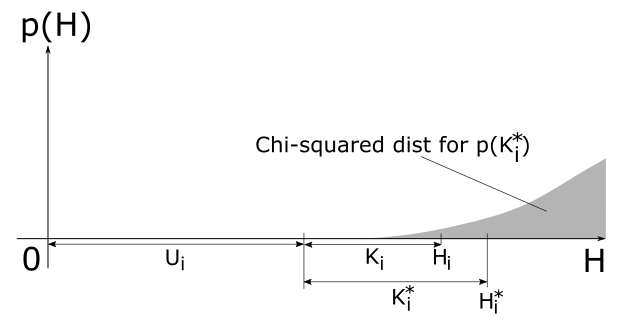
\includegraphics[width=10cm]{hmcmc_kinetic_energy_distribution.png}
\caption{Probability distribution over energy}
\label{fig:hmcmc_energy}
\end{figure}



\bibliography{sampling.bib}{}
\bibliographystyle{plain}

\end{document}


